%This is a very basic  BE PROJECT PRELIMINARY template.

%############################################# 
%#########Author :  PROJECT###########
%#########COMPUTER ENGINEERING############


\documentclass[oneside,a4paper,12pt]{report}
%\usepackage{showframe}
%\hoffset = 8.9436619718309859154929577464789pt
%\voffset = 13.028169014084507042253521126761pt


}

\pagestyle{fancy}
\fancyhead{}
\renewcommand{\headrulewidth}{0pt}
\footskip = 0.625in
\cfoot{}
\rfoot{}

\usepackage[]{hyperref}
\usepackage{tikz}
\usetikzlibrary{arrows,shapes,snakes,automata,backgrounds,petri}

\usepackage{tabularx}

\usepackage[nottoc,notlot,notlof,numbib]{tocbibind}
\usepackage[titletoc]{appendix}
\usepackage{titletoc}
\renewcommand{\appendixname}{Annexure}
%\renewcommand{\bibname}{References}

\setcounter{secnumdepth}{5}

\usepackage{float}
\usepackage{subcaption}
\usepackage{multirow}

\usepackage[ruled,vlined]{algorithm2e}

\pagestyle{fancy}
\begin{document}
\thispagestyle{empty}

\setlength{\parindent}{0mm}

\begin{center}

\addtolength{\topmargin}{-1.3in}
 \vspace*{1\baselineskip}
{\bfseries A PROJECT PHASE-I REPORT ON\\}
{\bfseries  ON \\}
 \vspace*{1\baselineskip}
{\bfseries \fontsize{16}{17} \selectfont  Cotton Crop Detection Using Machine Learning  \\ \vspace*{1\baselineskip}}
{\fontsize{12}{13} \selectfont SUBMITTED TOWARDS THE
 \\PARTIAL FULFILLMENT OF THE ACADEMIC REQUIREMENTS FOR THE SEMISTER VII \\

\vspace*{2\baselineskip}}
{\bfseries \fontsize{14}{10} \selectfont BACHELOR OF TECHNOLOGY\\ \vspace*{1\baselineskip}(Computer Engineering) \\
\vspace*{1\baselineskip}} 
{\bfseries \fontsize{14}{12} \selectfont Submitted by \\ 
\vspace*{0.5\baselineskip}} 
Rewa Narendra Desale  \hspace{22 mm}  Exam No: 21544920181124510056 \\
Khushboo Kiran Chaudhari \hspace{13 mm} Exam No: 21544920181124510057 \\
Harshada Vilas Pawar \hspace{23 mm}  Exam No: 21544920181124510070 \\
Arati Dhanraj Patil\hspace{29 mm} Exam No:  21544920181124510063\\
\vspace*{2\baselineskip}
{\bfseries \fontsize{14}{12} \selectfont Under The Guidance of \\  
\vspace*{1\baselineskip}} 
\bfseries \fontsize{12}{12}Prof. Bhushan Nandwalkar\vspace*{1\baselineskip}\\

\includegraphics[width=110 pt]{Update_logo_SVKM.jpg} \\
{\bfseries \fontsize{13}{15} \selectfont SHRI VILE PARLE KELAVANI MANDAL'S \\INSTITUTE OF TECHNOLOGY,DHULE 424001 \\
Affiliated To  \\
{\bfseries \fontsize{11}{15}\selectfont DR.BABASAHEB AMBEDKAR TECHNOLOGICAL UNIVERSITY, LONERE\\ Year:2024-2025 }

}
\end{center}

\newpage



\begin{figure}[ht]
\thispagestyle{empty}
\centering

\includegraphics[width=110 pt]{Update_logo_SVKM.jpg}
\end{figure}




{\bfseries \fontsize{16}{12} \selectfont \centerline{CERTIFICATE} 
\vspace*{2\baselineskip}} 

\centerline{This is to certify that the Project Entitled}
\vspace*{0.5\baselineskip} 


{\bfseries \fontsize{14}{12} \selectfont \centerline{ Cotton Crop Detection Using Machine Learning }
\vspace*{0.5\baselineskip}}

\centerline{Submitted by}
\vspace*{0.5\baselineskip} 
\centerline{Rewa Narendra Desale \hspace{22 mm}Exam No: 21544920181125410056}
\centerline{Khushboo Kiran Chaudhari \hspace{13 mm} Exam No: 21544920181124510057  } 
\centerline{Harshada Vilas Pawar \hspace{23 mm} Exam No: 21544920181124510070 }
\centerline{Arati Dhanaraj Patil  \hspace{25 mm} Exam No: 21544920181124510063 }
 \vspace*{0.5\baselineskip}
is a bonafide work carried out by Students under the supervision of Prof.Bhushan Nandwalkar and it
is submitted towards the partial fulfillment of the Academic requirements for the Semester VII (Computer Engineering).\\

\bgroup
\def\arraystretch{1}
\vspace*{2\baselineskip}
\begin{tabular}{c c }

Prof.Bhushan Nandwalkar &  \hspace{40 mm} Dr.Makrand Shahade \\								
Internal Guide   &  \hspace{40 mm} H.O.D \\
Dept. of Computer Engg.  &	\hspace{40 mm}Dept. of Computer Engg.  \\
\end{tabular}
%}
\vspace*{0.8\baselineskip} 
\begin{center}
%\fontsize{12}{19}\selectfont 
{
Dr.Nilesh Salunke \\
Principal\\
SVKM'S Institute of Technology,Dhule  
}
\end{center}
\\\\
\vspace*{1\baselineskip}
Signature of Internal Examiner \hspace{22 mm} Signature of External Examiner

\newpage
\begin{center}
\textbf{PROJECT APPROVAL SHEET}
\end{center}
\begin{center}
 A Project Title
 \end{center} \\
\begin{center}
Cotton Crop Detection Using Machine Learning
\end{center}\\
\begin{center}
Is successfully completed by 
\end{center}
\vspace*{0.5\baselineskip} 
\centerline{Rewa Narendra Desale \hspace{22 mm} Exam No: 21544920181125410056} 
\centerline{Khushboo Kiran Chaudhari \hspace{13 mm} Exam No: 21544920181124510057} 
\centerline{Harshada Vilas Pawar \hspace{23 mm} Exam No: 21544920181124510070}
\centerline{Arati Dhanaraj Patil  \hspace{25 mm} Exam No: 21544920181124510063}
 \vspace*{0.5\baselineskip}
\begin{center}
 at
 \end{center} 
 \begin{center}
 DEPARTMENT OF COMPUTER ENGINEERING
 \end{center}
 \begin{center}
 SHRI VILE PARLE KELAVANI MANDAL'S INSTITUTE OF TECHNOLOGY,DHULE
 \end{center}
 \begin{center}
 DR.BABASAHEB AMBEDKAR TECHNOLOGICAL UNIVERSITY,LONERE
 \end{center}
 
 \begin{center}
 ACADEMIC YEAR 2024-2025
 \end{center}
 \vspace*{3\baselineskip}}
 \begin{tabular}{c c }
Prof.Guide Name &  \hspace{30 mm} Prof.Bhushan Nandwalkar \\								
Internal Guide   &  \hspace{30 mm} Project Coordinator \\
Dept. of Computer Engg.  &	\hspace{30 mm}Dept. of Computer Engg.  \\
\end{tabular}
\pagenumbering{roman}







{  {\newpage {\bfseries \fontsize{14}{12} \selectfont \centerline{Acknowledgments} 

\vspace*{2\baselineskip}} \setlength{\parindent}{11mm} }
{ \setlength{\parindent}{0mm} }

\textmd{It gives us great pleasure in presenting the preliminary project report 
on {\bfseries \fontsize{12}{12} \selectfont `B.Tech. PROJECT TITLE'}.}
\vspace*{1.5\baselineskip}

 \textmd{We would like to take this opportunity to thank our internal project guide 
 \textbf{Prof. Guide Name} for giving us all the help and guidance we needed. We really grateful to him for his kind support.His valuable suggestions were very helpful.} \vspace*{1.5\baselineskip}

 \textmd{We also grateful to \textbf{Dr.Makarand Shahade},H.O.D.Department of Computer Engineering for his indispensable support and suggestions.}
\vspace*{1.5\baselineskip}

\textmd{We express our heartfelt thanks to Hon.Principal  \textbf{Dr.Nilesh Salunke} for providing various infrastructural facility ,other resources, encouragement and support in academics.}\vspace*{1.5\baselineskip}

\textmd{We would like to thanks to all teaching and non-teaching staff of Department of Computer Engineering for their encouragement and suggestions for our project.Our sincere thanks to all our friends, who helped us directly or indirectly in completing this project work.We would like to express our appreciation for the wonderful experience while completions of this project work.}
\vspace*{3\baselineskip} \\
\begin{tabular}{p{8.2cm}c}
&Student Name1\\
&Student Name2\\
&Student Name3\\
&Student Name4\\
&(B.Tech Computer Engg.)
%}
\end{tabular}
		
{  \newpage {\bfseries \fontsize{14}{12} \selectfont \centerline{Abstract} 
\vspace*{2\baselineskip}} \setlength{\parindent}{11mm} }
{ \setlength{\parindent}{0mm} }
Please Write here One Page Abstract. It should mainly include introduction, motivation,outcome and innovation if any.






 \tableofcontents
 \listoffigures 
 \listoftables




\chapter{Synopsis}
\pagenumbering{arabic}
\section{Project Title}
\begin{itemize}
\item Project Title
\end{itemize}


\section{Domain of Project}  
\begin{itemize}
\item Domain of Project
\end{itemize}

\section{Problem Statement}
\begin{itemize}
\item Write problem statement in detail
\end{itemize}

\section{Objectives and Expected Outcomes }  
\begin{itemize}
\item Objectives and Expected Outcomes
\end{itemize}

\chapter{Introduction}
\section{Overview of Project Domain}
\begin{itemize}
\item Overview of Project Domain
\end{itemize}


\section{Project Purpose and Applicability}  
\begin{itemize}
\item Project Purpose and Applicability
\end{itemize}

\section{Scope of Project}
\begin{itemize}
\item Scope of Project
\end{itemize}



\chapter{Literature Survey }
\section{Related Work Done }
\item Explain Referred Papers for paper in paragraph. 
\section{Limitation of Existing System }
\item Explain Limitations of Existing System
\section{Motivation of Proposed System }
\item


\chapter{Project Implementation Plan for Phase-I}
 \section{Project Schedule} 
 \subsection{Project Task Set}
 Major Tasks in the Project stages are:
\begin{itemize}
  \item Task 1: 
  \item Task 2: 
  \item Task 3: 
  \item Task 4: 
  \item Task 5: 
\end{itemize}

 \subsection{Time Line Chart}
 A project timeline chart is presented. This may include a time line for the phase-I of project.


\chapter{Project Requirement Specification  }

\section{Hardware and Software Requirement }
\ Hardware Requirement:

\begin{table}[!htbp]
\begin{center}
\def\arraystretch{1.5}
  \begin{tabular}{| c | c | c | c |}
\hline
Sr. No. &	Parameter &	Minimum Requirement & Justification \\
\hline
1 &	CPU Speed &	 2 GHz  & Remark Required\\
\hline
2 &	RAM  &	3 GB &  Remark Required\\
 \hline
\end{tabular}
 \caption { Hardware Requirements }
 \label{tab:hreq}
\end{center}

\end{table}


\ Software Requirement : 
\begin{enumerate}
\item Operating System: 
\item Programming Language
\end{enumerate}


\section{Functional Requirement}

\section{Non Functional Requirement }
\begin{itemize}
	\item	Interface Requirements
	\item	Performance Requirements
   
\end{itemize} 

\section{Data Set Description/Database Schema }
  

\chapter{Proposed System}
\section{System Design and Architecture}
      Draw overall system and explain it's all module with functionality and explanation of used algorithms(Pseudo Code). 
      
  \section{Data Flow Diagram}
  Draw Data Flow Diagrams. Example is given below
  
    \subsection {DFD Level 0}
  \begin{center}
	\begin{figure}[!htbp]
		\centering
		\fbox{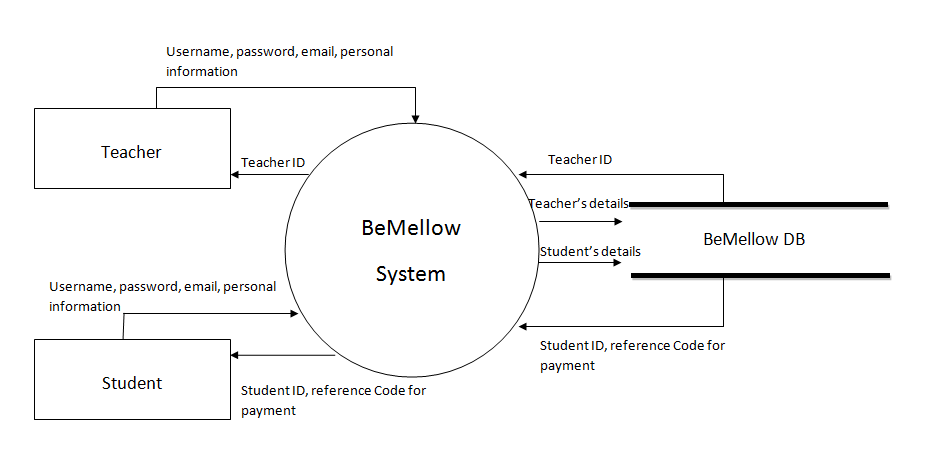
\includegraphics[width=350pt]{DFD Level 0.png}}
	  \caption{Data Flow Diagram Level 0}
	  \label{fig:DFD Level 0}
	\end{figure}
\end{center}  

\subsection {DFD Level 1}
  \begin{center}
	\begin{figure}[!htbp]
		\centering
		\fbox{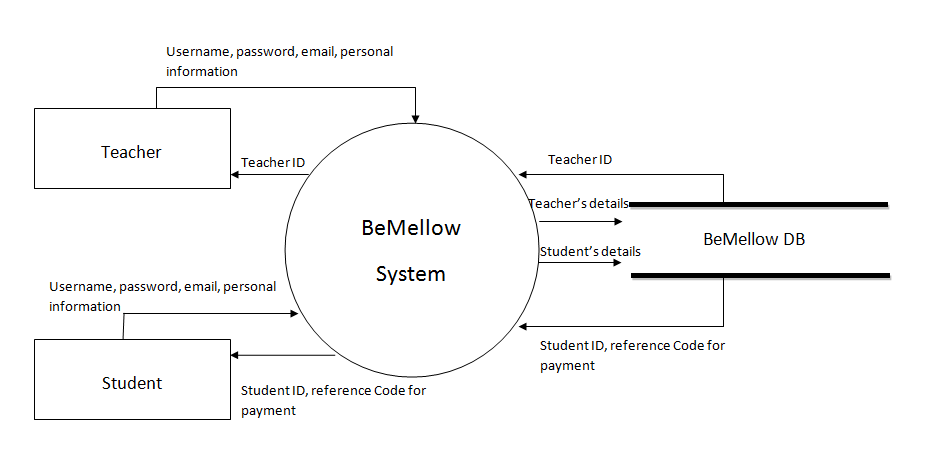
\includegraphics[width=350pt]{DFD Level 0.png}}
	  \caption{Data Flow Diagram Level 1}
	  \label{fig:DFD Level 1}
	\end{figure}
\end{center}  


\subsection {DFD Level 2}
  \begin{center}
	\begin{figure}[!htbp]
		\centering
		\fbox{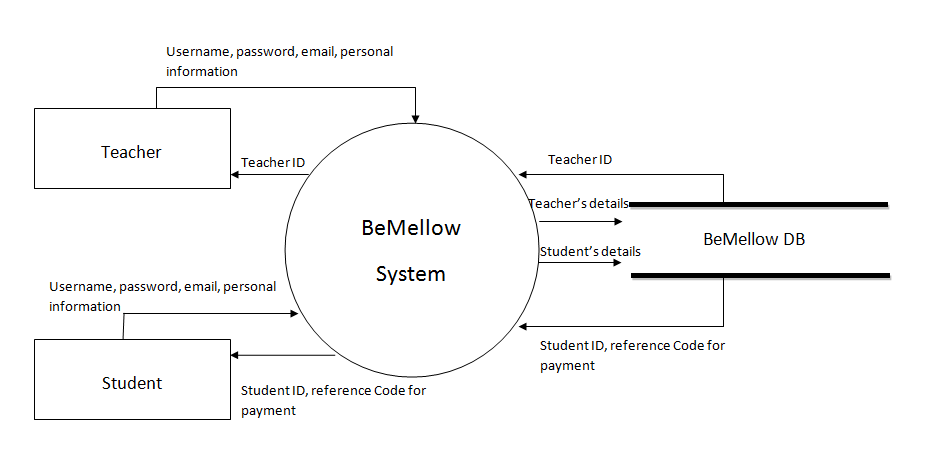
\includegraphics[width=350pt]{DFD Level 0.png}}
	  \caption{Data Flow Diagram Level 2}
	  \label{fig:DFD Level 1}
	\end{figure}
\end{center}  


  \section{UML Diagrams}
  \subsection{Use Case Diagram}
  
   \begin{center}
	\begin{figure}[!htbp]
		\centering
		\fbox{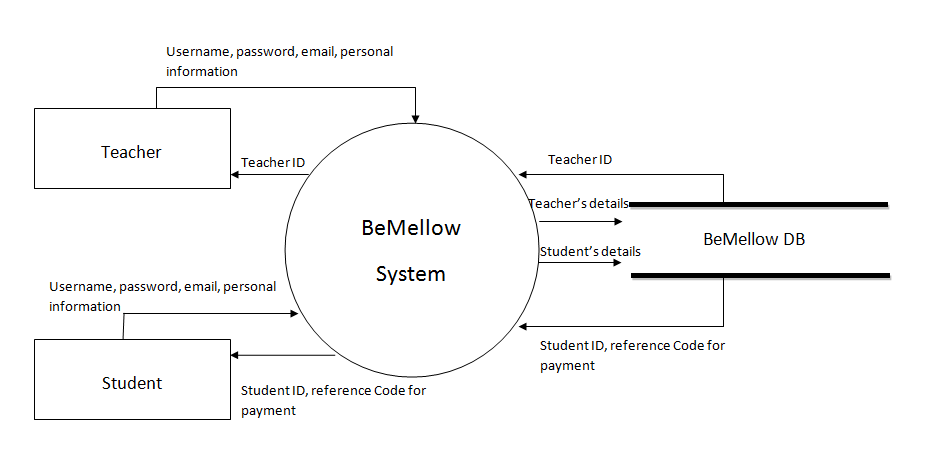
\includegraphics[width=350pt]{DFD Level 0.png}}
	  \caption{Use Case Diagram}
	  \label{fig:Use Case}
	\end{figure}
\end{center} 
  
   
  \subsection{Sequence Diagram(if Required)}
       \begin{center}
	\begin{figure}[!htbp]
		\centering
		\fbox{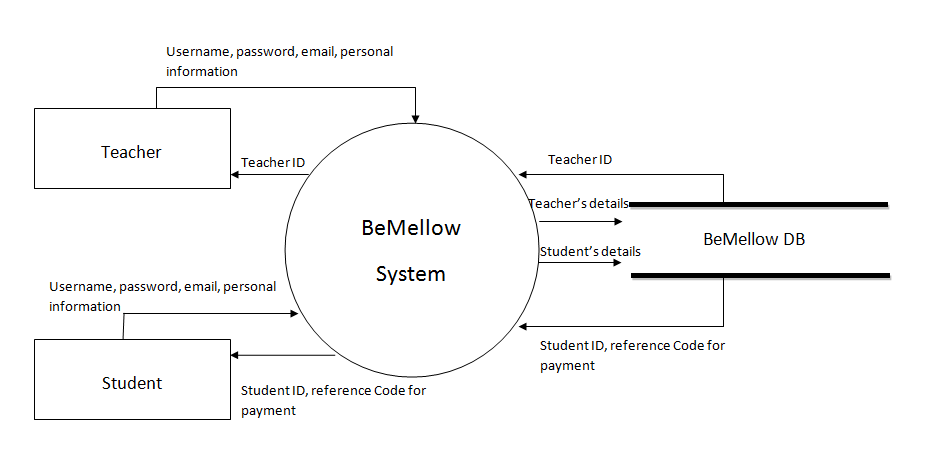
\includegraphics[width=350pt]{DFD Level 0.png}}
	  \caption{Sequence Diagram}
	  \label{fig:Sequence Diagram}
	\end{figure}
\end{center} 
  
   \subsection{Class Diagram(if Required)}
   
   \begin{center}
	\begin{figure}[!htbp]
		\centering
		\fbox{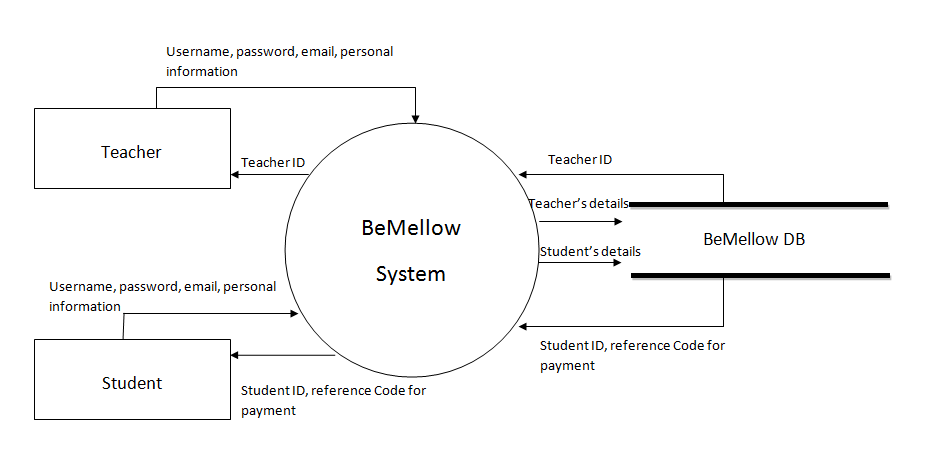
\includegraphics[width=350pt]{DFD Level 0.png}}
	  \caption{Class Diagram}
	  \label{fig:Class Diagram}
	\end{figure}
\end{center} 
   
   
    \section{System Implementation}
    Complete Module Screenshots or Code Snippet(30 percent Completed work)  

   
   

     
   
  



     
 \chapter{Conclusion and future scope}
Write  summary , conclusion and future scope
 }


% \bibliographystyle{plain}

%\bibliographystyle{ieeetr}
%\bibliography{biblo}

\begin{appendices}

\chapter{References}
[1] Sachchidanand Singh, Nirmala Singh“Big Data Analytics” International Conference on Communication,Information & Computing Technology (ICCICT), Oct. 19-20, Mumbai, India,pp.1-4.2010.


% \chapter{ALGORITHMIC DESIGN}





\end{enumerate}
\end{appendices}


\end{document}
